% Crucial Preamble
\documentclass[12pt,letterpaper]{article} \usepackage{amsmath} \usepackage{graphicx} \usepackage[margin=1in]{geometry} \usepackage{longtable}  \usepackage{amssymb}

% Extra Preamble
\usepackage{fancyhdr} \usepackage{enumitem} \usepackage{float} \usepackage{soul}
\usepackage{multicol} \usepackage[compact]{titlesec} \usepackage{listings}


% frames with display breaks
\usepackage{mdframed}
\allowdisplaybreaks

% change spacing
\usepackage{setspace}
\setlength{\parskip}{0.4\baselineskip}

% Remove paragraph indentation
\setlength{\parindent}{0pt}

% Reduce space before and after section headings
%\titlespacing*{\section}{0pt}{0.1\baselineskip}{0.2\baselineskip}

% changes font
%\renewcommand{\familydefault}{\sfdefault}

% adds header and footer
\pagestyle{fancy}
\fancyhead{} \fancyhead[C]{SEG 2106 Cheat Sheet} \fancyhead[L]{SEG2106} \fancyhead[R]{Owen Daigle}
\fancyfoot{} \fancyfoot[C]{\thepage}


\begin{document}
	
	\begin{center}
		\Large\textbf{SEG 2106 Cheat Sheet} \\
		\vspace{0.5em}
	\end{center}
	
	\section {Software Development Processes}
	\subsection{Black and White Box}
	The \textbf{black box} process gets the requirements for a project, then the team works on the project for a set period of time, and produces a product. 
	
	Thie \textbf{white box} process is similar to the black box process except for the stakeholders periodically check up on the project to provide \textbf{feedback}. 
	
	\subsection{Models}
	The \textbf{waterfall model} sequentially does domain analysis, gets requirements, makes a design, then tests and finally deploys. 
	
	This is very easy and good under ideal circumstances, but in the real word this is rarely used since \textbf{circumstances are rarely ideal}. Often stakeholders do not effectively communicate requirements to developers, or the requirements change. 
	
	We can modify the waterfall by adding \textbf{feedback} into the loop at each stage, so if we need to change something, we do not have to redo the whole project. This is an \textbf{agile development process}. 
	
	\section{Requirements Modeling}
	To get the requirements for a project, we need to analyse the domain the software will be used in. We need to understand the domain that the users are in so we can create software that works for the users. 
	
	We can make UML class diagrams for a system and all its parts. 
	
	\subsection{Requirements}
	We need to interview the stakeholders to figure out what they want. These are usually lots of sentences that say in general non technical terms what the system needs to do. 
	
	A system will have lots of use cases. Each use case is a "thing" that the user wants to do. Such as "create text file" or "delete file".
	
	We can create a use case diagram which is a diagram depicting all the use cases, and what user does that use case. 
	
	For each use case, we have the following information:
	\begin{itemize}[noitemsep]
		\item Actors
		\item Summary
		\item Precondition (does the system have to be in a specific state to do this use case?)
		\item Main Sequence (Sequence of what the user does and how the system responds)
		\item Alternative Sequences (Basically modifications to the main sequence depending on other events.)
		\item Postcondition (What state the system is in after the use case. )
	\end{itemize}

	\begin{mdframed}
		\textbf{Ex. } 
		% put example of use case diagram
	\end{mdframed}

	\textbf{Functional Requirements} are things that the system is supposed to do. 
	
	\textbf{Non Functional Requirements} are more about how the system is supposed to do something. Such as the system "must complete action in less than 5 seconds" or the system "must store password as encrypted".
	
	A \textbf{user story} is a more general form of a use case.
 	
	\section{Behavioral Modeling}
	
	\subsection{UML Activity Diagrams}
	This is a diagram that models behaviour of a system. They are good to model concurrent behaviour. 
	
	\begin{mdframed}
		\textbf{Ex. } 
		% put ex of activity
	\end{mdframed}
	
	\subsection{UML State Machines}
	This is a high level diagram that models the states of a certain part of a system. It is good at working with a single object/part. 
	
	\subsection{Petri Nets}
	This is a diagram that is good for modeling complex concurrent behaviour. They get very complex very fast though, so they are not great for large projects unless we have a large time budget. 
	
	A petri net works off of tokens. Tokens can trigger transitions that will cause tokens to move locations, add new tokens, or consume tokens. 
	
	A petri net is \textbf{bounded} if the number of tokens cannot exceed a finite amount. Conversely, a petri net is \textbf{unbounded} if \textit{there exists at least one} way for a petri net to create an infinite number of tokens. 
	
	A petri net is \textbf{alive} if there is always at \textit{least one transition } that can be fired from any point. Conversely, if there is any reachable combination where the system cannot do anything else (it dies), the petri net is not alive. 
	
	\begin{mdframed}
		\textbf{Ex. }
		% put ex of petri with boundedness and aliveness calculation
	\end{mdframed}
	
	\subsection{Specification and Description Language (SDL)}
	SDL has 3 main hierarchical levels. System, Block, and Process. 
	
	A system has one or more blocks interconnected with other. 
	
	A process is a state machine that has states and transitions, kind of like a UML state machine. 
	
	\section{Lexical Analysis}
	This is one part of a compiler. It checks that all the words in the program are \textbf{part of the language. }
	
	For example, if the language is java, "print" is not a word, but "if" and "System.out" are words. 
	
	Regular Expressions are used to do this. 
	
	\subsection{Alphabet}
	The \textbf{alphabet} are all the characters that we are working with. If a letter not in the alphabet is found, then the string is not accepted. 
	
	\begin{mdframed}
		\textbf{Ex. } If the alphabet is {a,b,c} then:
		
		"aaa" may be good
		
		"aaabbbbcccc" may be good
		
		"aaabbbcccddd" is NOT good since "d" is not in the alphabet. 
		
	\end{mdframed}

	\subsection{Operations}
	Union is the or operator. A|B means A or B
	
	Concatenation is 2 consecutive strings. AB means the string AB, not BA, AA, BB...
	
	Kleene Closure is the set of all strings that can be created from 0 or more strings defined. (aa)* means kleene closure of (aa) which is "", "aa", "aaaa", "aaaaaa", but not "a", "ab", "aaa"...
	
	Positive closure is like kleene closure but excludes the empty string. So, (aa)+ is the positive closure of (aa) which is "aa", "aaaa", ... Note the exclusion of "".
	
	\subsection{NFA}
	Non-deterministic Finite Automata (NFA) are a type of machine that model a regular expression. These have multiple states that are connected to each other with transitions. These transitions can be either $\epsilon$ (the empty string) or any value in the alphabet. 
	
	We use the following rules to convert a regular expression (regex) into an NFA:
	\begin{center}
		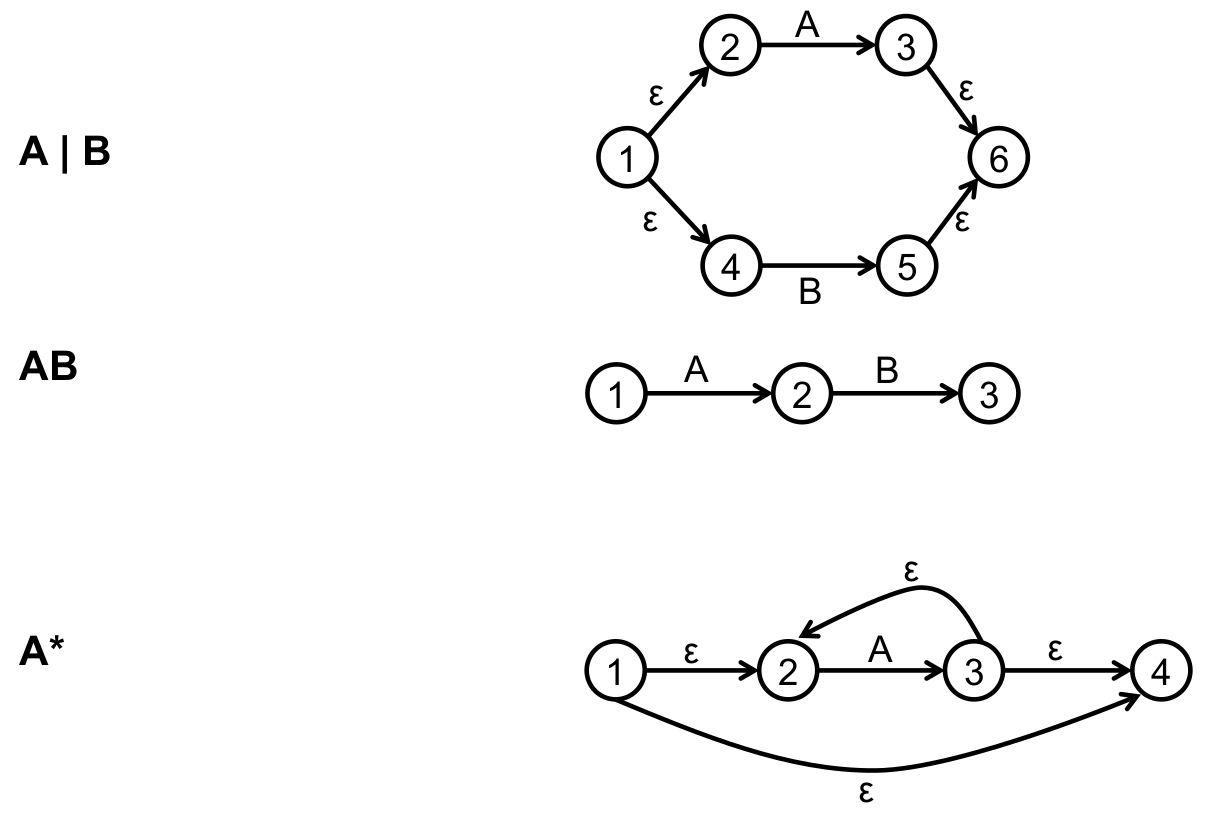
\includegraphics[width=0.7\linewidth]{nfa-rules}
	\end{center}

	We can combine these together to model more complicated REGEX such as (a|b)* which is just the A* design, but instead of A, we substitute the A|B design.
	
	\begin{mdframed}
		\textbf{Ex. } Find the NFA of \_\_\_\_\_
		% fill in later
	\end{mdframed}
	
	\subsection{DFA}
	NFA is easy to get, but it is hard for the computer to interpret it. This is where the Deterministic Finite Automata (DFA) comes into play. We create this using the \textbf{subset construction algorithm} on a NFA. In worst case scenario, we could have $2^n$ states where $n$ is the number of states in NFA.
	
	We have 2 functions.
	
	$\epsilon$-closure(S) is the state of the system that is reached by all epsilon transitions from state S. 
	
	move(S,a) will be the state the system is in after starting in state S and then taking the transition a.
	
	Basically, we make a table with all the states of the system (up to $2^n$) as rows, and colums for each letter of the alphabet. Then we perform move for each row (S), and each column (a)
	
	\begin{mdframed}
		\textbf{Ex. } Get the DFA of the following NFA through the subset construction algorithm:
		% fill in later
	\end{mdframed}
	
	\section{Syntax Analysis}
	% for later
	
	\section{Concurrency}
	% for later

	
\end{document}